Käytännössä kaksi ryhmää teknologioille: käyttäjädatan tallennus ja tunnistautumisprotokollat.

Käyttäjädatan tallennus
- passwd (ts tiedosto levyllä tms)
- tietokanta
- AD-kannat (LDAP)

---> käyttäjän datan abstraktoinnin tarve, ehkä mainita, että käyttäjädatan backendejä voi käytännössä olla monta erilaista. Esim. LDAP:n rinnalla tietokannat.

Enivei, luvun pääpaino on protokollissa. Esitellään historia kerberos -> saml -> oauth ja päädytään oauthiin, tarkemmin versioon 2.

Tunnistautumiseen liittyvien käsitteiden läpikäynti ennen protokollien yksityiskohtaista esittelyä auttaa tunnistautumiseen liittyvien periaatteiden hahmottamista. Käsitteet ovat yleisluontoisia ja eivätkä kosketa vain tiettyjä protokollaa. Protokollien yhteydessä käytetään käsitteitä asiakasohjelma, tunnistautumispalvelu, suojattu resurssi, valtuutustieto (credentials), valtuutusavain (authorization code) ja pääsyvaltuutus (access token) \cite{nisti}.

Asiakasohjelmalla tarkoitetaan web-palvelun käyttäjän pääteohjelmaa, jolla hän kirjautuu web-palveluun käyttäen keskitettyä tunnistautumispalvelua. Käytännössä asiakasohjelma on web-palvelun tapauksessa käyttäjän WWW-selain, joka pystyy tekemään uudelleenohjauksia sivustolta toiselle. Uudelleenohjaus on HTTP-protokollan perustoiminnallisuutta, joten mikä tahansa HTTP/1.1-standardin WWW-selain käy asiakasohjelmaksi \cite{rfc2616}.

Tunnistautumispalvelu on web-palvelu, johon käyttäjä ohjataan tekemään tunnistautuminen. Onnistuneen tunnistautumisen jälkeen tunnistautumispalvelu ohjaa asi\-a\-kas\-oh\-jel\-man takaisin tunnistautumista pyytäneen palvelun määrittelemään osoitteeseen \cite{nisti}. Avoimen Internetin puolella tunnistautumispalvelu voi olla esimerkiksi Facebook tai LinkedIn.

Tunnistautumisprotokollien yhteydessä suojatulla resurssilla tarkoitetaan resurssia, jonka käyttö vaatii tunnistautumisen ja käyttöoikeuden. Yleisessä tapauksessa suojatulla resurssilla tarkoitetaan yksittäistä resurssia (käyttäjän valokuvaa), johon halutaan asettaa pääsyrajoituksia \cite{nisti}. Tämän tutkielman puitteissa suojatulla resurssilla tarkoitetaan tunnistautumista vaativaa web-palvelua.

Valtuutustieto koostuu yksilöivästä tunnisteesta ja siihen liittyvästä salaisesta avaimesta. Tämän tutkielman puitteissa valtuutustiedolla tarkoitetaan käyttäjän tunnusta ja salasanaa.

Kirjauduttuaan sisään tunnistautumispalvelimelle, käyttäjä saa valtuutusavaimen, jonka hän lähettää eteenpäin suojatun resurssin omistajalle. Valtuutusavain ei pidä sisällään käyttäjän valtuutustietoja, vaan ainoastaan tunnistautumispalvelin osaa lukea sen \cite{nisti}. Saatuaan valtuutusavaimen käyttäjältä voi suojatun resurssin omistaja hakea pääsyvaltuuden käyttäjän tietoihin tunnistautumispalvelusta.

Pääsyvaltuutus on tunnistautumispalvelimelta saatava yksilöivä tunniste, jonka avulla suojatun resurssin omistaja voi pyytää käyttäjän tiedot tunnistautumispalvelulta. Pääsyvaltuutus on voimassa tietyn ajan, jonka jälkeen se täytyy uusia tunnistautumispalvelimella \cite{nisti}. Pääsyvaltuutusta voidaan käyttää myös tunnistautumispalvelusta erillään olevien resurssien valtuuttamiseen. Esimerkiksi web-sovellus voi hakea tunnistautumispalvelulta pääsyvaltuuden, jolla hän hakee valokuvia valokuvien jakopalvelusta \cite{facebook}.
\subsection{Käyttäjädata}
Tunnistautumiseen liittyvien käsitteiden läpikäynti ennen protokollien yksityiskohtaista esittelyä auttaa tunnistautumiseen liittyvien periaatteiden hahmottamista. Käsitteet ovat yleisluontoisia ja eivätkä kosketa vain tiettyjä protokollaa. Protokollien yhteydessä käytetään käsitteitä asiakasohjelma, tunnistautumispalvelu, suojattu resurssi, valtuutustieto (credentials), valtuutusavain (authorization code) ja pääsyvaltuutus (access token) \cite{nisti}.

Asiakasohjelmalla tarkoitetaan web-palvelun käyttäjän pääteohjelmaa, jolla hän kirjautuu web-palveluun käyttäen keskitettyä tunnistautumispalvelua. Käytännössä asiakasohjelma on web-palvelun tapauksessa käyttäjän WWW-selain, joka pystyy tekemään uudelleenohjauksia sivustolta toiselle. Uudelleenohjaus on HTTP-protokollan perustoiminnallisuutta, joten mikä tahansa HTTP/1.1-standardin WWW-selain käy asiakasohjelmaksi \cite{rfc2616}.

Tunnistautumispalvelu on web-palvelu, johon käyttäjä ohjataan tekemään tunnistautuminen. Onnistuneen tunnistautumisen jälkeen tunnistautumispalvelu ohjaa asi\-a\-kas\-oh\-jel\-man takaisin tunnistautumista pyytäneen palvelun määrittelemään osoitteeseen \cite{nisti}. Avoimen Internetin puolella tunnistautumispalvelu voi olla esimerkiksi Facebook tai LinkedIn.

Tunnistautumisprotokollien yhteydessä suojatulla resurssilla tarkoitetaan resurssia, jonka käyttö vaatii tunnistautumisen ja käyttöoikeuden. Yleisessä tapauksessa suojatulla resurssilla tarkoitetaan yksittäistä resurssia (käyttäjän valokuvaa), johon halutaan asettaa pääsyrajoituksia \cite{nisti}. Tämän tutkielman puitteissa suojatulla resurssilla tarkoitetaan tunnistautumista vaativaa web-palvelua.

Valtuutustieto koostuu yksilöivästä tunnisteesta ja siihen liittyvästä salaisesta avaimesta. Tämän tutkielman puitteissa valtuutustiedolla tarkoitetaan käyttäjän tunnusta ja salasanaa.

Kirjauduttuaan sisään tunnistautumispalvelimelle, käyttäjä saa valtuutusavaimen, jonka hän lähettää eteenpäin suojatun resurssin omistajalle. Valtuutusavain ei pidä sisällään käyttäjän valtuutustietoja, vaan ainoastaan tunnistautumispalvelin osaa lukea sen \cite{nisti}. Saatuaan valtuutusavaimen käyttäjältä voi suojatun resurssin omistaja hakea pääsyvaltuuden käyttäjän tietoihin tunnistautumispalvelusta.

Pääsyvaltuutus on tunnistautumispalvelimelta saatava yksilöivä tunniste, jonka avulla suojatun resurssin omistaja voi pyytää käyttäjän tiedot tunnistautumispalvelulta. Pääsyvaltuutus on voimassa tietyn ajan, jonka jälkeen se täytyy uusia tunnistautumispalvelimella \cite{nisti}. Pääsyvaltuutusta voidaan käyttää myös tunnistautumispalvelusta erillään olevien resurssien valtuuttamiseen. Esimerkiksi web-sovellus voi hakea tunnistautumispalvelulta pääsyvaltuuden, jolla hän hakee valokuvia valokuvien jakopalvelusta \cite{facebook}.
\subsubsection{passwd}
Vanha kunnon /etc/passwd, tästä tunnistautuminen on varmaan lähtenyt käyntiin. Ikävää, kun webiin tunnistautuessa täytyy olla tunnus kyseisellä koneella ja muutenkin ei ole hyvä kun tunnukset siirtyy verkkoa pitkin.
\subsubsection{Relaatiotietokannat}
Käyttäjätietokannat, relaatiokannat lähinnä, ehkä NoSQL.
\subsubsection{LDAP}
Lähteet: Howes, T. A., The Lightweight Directory Access Protocol: X.500 Lite. CITI
Technical Report 95–8, University of Michigan, 1995. \cite{howes} \\
rfc:t 4510-4513 (ainakin 4513 "Authentication Methods and Security Mechanisms" kiinnostaa)

Lightweight Directory Access Protocol (LDAP) on X.500 OSI-standardiin perustuva hakemistopalvelu, jota käytetään yleisesti käyttäjätiedon tallennukseen [TODO: lähde]. 1990-luvulla TCP/IP-mallin syrjäytettyä OSI-mallin, myös DAP kävi vanhanaikaiseksi \cite{howes}. Korvaajaksi on noussut LDAP, josta käytetään myös nimeä X.500 Lite \cite{howes}.

LDAP:ssa asiakassovellukset (directory user agent, DUA) keskustelevat puumalliin perustuvan hakemistopalvelimen (directory system agent, DSA) kanssa käyttäen määriteltyä protokollaa (directory access protocol, DAP) \cite{howes}. Asiakassovellukset voivat hakea hakemistopalvelimesta tietoa suodattimiin (filter) perustuvalla lukuoperaatiolla. Suodattimessa voidaan määritellä raja-arvot attribuutin arvolle tai hakea avainsanoilla attribuuteista.

LDAP-tietuille voidaan määritellä pakollisten attribuuttien (esim. etu- ja sukunimi) lisäksi valinnaisia attribuutteja. Tietueet on järjestetty puuhun niiden yksilöivän nimen (distinguished name, DN) mukaan ja ne voi olla hajautettu usealle palvelimelle. Suhteellinen nimi (relative distinguished name, RDN) identifioi tietueen omalla hierarkiatasollaan.

LDAP-tietueella voi olla tunnus sekä salasana ja LDAP-palvelinta voidaan käyttää käyttäjän tunnistautumiseen [TODO: lähde, ehkä rfc4513].

TODO: lisää tekstiä

\subsubsection{Käyttäjädatan abstraktointi}
Tutkimuksen kannalta abstraktointi on oleellista, oikeastaan sillä ei ole ison kuvan kannalta merkitystä, että onko siellä taustalla tietokanta, tiedosto, ldap vai mikä.
\subsection{Rajapintaprotokollat}
Tunnistautumiseen liittyvien käsitteiden läpikäynti ennen protokollien yksityiskohtaista esittelyä auttaa tunnistautumiseen liittyvien periaatteiden hahmottamista. Käsitteet ovat yleisluontoisia ja eivätkä kosketa vain tiettyjä protokollaa. Protokollien yhteydessä käytetään käsitteitä asiakasohjelma, tunnistautumispalvelu, suojattu resurssi, valtuutustieto (credentials), valtuutusavain (authorization code) ja pääsyvaltuutus (access token) \cite{nisti}.

Asiakasohjelmalla tarkoitetaan web-palvelun käyttäjän pääteohjelmaa, jolla hän kirjautuu web-palveluun käyttäen keskitettyä tunnistautumispalvelua. Käytännössä asiakasohjelma on web-palvelun tapauksessa käyttäjän WWW-selain, joka pystyy tekemään uudelleenohjauksia sivustolta toiselle. Uudelleenohjaus on HTTP-protokollan perustoiminnallisuutta, joten mikä tahansa HTTP/1.1-standardin WWW-selain käy asiakasohjelmaksi \cite{rfc2616}.

Tunnistautumispalvelu on web-palvelu, johon käyttäjä ohjataan tekemään tunnistautuminen. Onnistuneen tunnistautumisen jälkeen tunnistautumispalvelu ohjaa asi\-a\-kas\-oh\-jel\-man takaisin tunnistautumista pyytäneen palvelun määrittelemään osoitteeseen \cite{nisti}. Avoimen Internetin puolella tunnistautumispalvelu voi olla esimerkiksi Facebook tai LinkedIn.

Tunnistautumisprotokollien yhteydessä suojatulla resurssilla tarkoitetaan resurssia, jonka käyttö vaatii tunnistautumisen ja käyttöoikeuden. Yleisessä tapauksessa suojatulla resurssilla tarkoitetaan yksittäistä resurssia (käyttäjän valokuvaa), johon halutaan asettaa pääsyrajoituksia \cite{nisti}. Tämän tutkielman puitteissa suojatulla resurssilla tarkoitetaan tunnistautumista vaativaa web-palvelua.

Valtuutustieto koostuu yksilöivästä tunnisteesta ja siihen liittyvästä salaisesta avaimesta. Tämän tutkielman puitteissa valtuutustiedolla tarkoitetaan käyttäjän tunnusta ja salasanaa.

Kirjauduttuaan sisään tunnistautumispalvelimelle, käyttäjä saa valtuutusavaimen, jonka hän lähettää eteenpäin suojatun resurssin omistajalle. Valtuutusavain ei pidä sisällään käyttäjän valtuutustietoja, vaan ainoastaan tunnistautumispalvelin osaa lukea sen \cite{nisti}. Saatuaan valtuutusavaimen käyttäjältä voi suojatun resurssin omistaja hakea pääsyvaltuuden käyttäjän tietoihin tunnistautumispalvelusta.

Pääsyvaltuutus on tunnistautumispalvelimelta saatava yksilöivä tunniste, jonka avulla suojatun resurssin omistaja voi pyytää käyttäjän tiedot tunnistautumispalvelulta. Pääsyvaltuutus on voimassa tietyn ajan, jonka jälkeen se täytyy uusia tunnistautumispalvelimella \cite{nisti}. Pääsyvaltuutusta voidaan käyttää myös tunnistautumispalvelusta erillään olevien resurssien valtuuttamiseen. Esimerkiksi web-sovellus voi hakea tunnistautumispalvelulta pääsyvaltuuden, jolla hän hakee valokuvia valokuvien jakopalvelusta \cite{facebook}.
\subsubsection{Kerberos}
Lähteet:
Enhancing Distributed Web Security Based on Kerberos Authentication Service
Secure Secret-Key Management of Kerberos Service

Kerberos-protokolla on alunperin MIT:ssa kehitetty tunnistautumisprotokolla, jonka nykyisin käytössä oleva versio 5 julkaistiin alunperin syyskuussa 1993 ja päivitettynä heinäkuussa 2005 [RFC4120]. Se on yleisesti käytössä erilaisissa UNIX-pohjaisissa käyttöjärjestelmissä ja myös Microsoft on käyttänyt sitä oletus-tunnistautumismekanismina Windows 2000:sta lähtien [RFC3244].

Protokollan osapuolia ovat käyttäjä, luotettava kolmas osapuoli ja palvelu, joka vaatii tunnistautumisen. Luotettava kolmas osapuoli on tyypillisesti avaintenjakopalvelin (KDC, Key Distribution Center), joka tunnistaa käyttäjän ja myöntää lipun tunnistautuneelle käyttäjälle. Myönnettyyn lippuun on merkattu palvelu, johon sitä voidaan käyttää ja aikaleima, jonka ajan se on voimassa. Käyttäjä antaa lipun tunnistautumista vaativalle palvelimelle, joka tarkistaa omalla avaimellaan käyttäjän tunnisteen ja aikaleiman, joiden perusteella se myöntää pääsyn palveluun.

Keskitetty tunnistautuminen hajautettuihin järjestelmiin voidaan toteuttaa Kerberos-protokollalla [Enhancing...]. Kerberos on luonteeltaan sopiva hajautettuihin järjestelmiin, koska avaintenjakopalvelin voi jakaa lippuja kaikkiin järjestelmiin, joiden kanssa se on vaihtanut salausavaimet. Tunnistautumispalvelin on tilaton, jolloin sen suorituskykyä voidaan parantaa tarvittaessa skaalaamalla, joten tunnistautumispalvelin voi palvella suurta määrää käyttäjiä [Enhancing...].

Tunnistautumisessa käytetyt yksityiset avaimet tallennetaan tietokantaan, jolloin on riskinä, että kolmas osapuoli saattaa päästä käsiksi näihin avaimiin ja pystyä allekirjoittamaan lippuja. Jakamalla salaiset avaimet osiin ja hajauttaa se avaintenjakopalvelimeen, tunnistautumista vaativalle palvelimelle ja näiden välillä käytetylle reitittimelle [Secure Secret-Key...], voidaan parantaa protokollan luotettavuutta. Tämä tekee siitä mahdollisen vaihtoehdon käytetyksi menetelmäksi keskitettyyn tunnistautumiseen hajautetuissa järjestelmistä.

\subsubsection{SAML}
Security Assertion Markup Language (SAML) on OASIS-komitean määrittelemä XML-pohjainen avoin standardi tunnistautumiseen ja pääsynhallintaan \cite{saml_spec}. Standardin versio 1.0 julkaistiin marraskuussa 2002 ja versio 2.0 maaliskuussa 2005. Version 2.0:n viimeisin korjattu versio 5 julkaistiin helmikuussa 2012.

SAML määrittelee XML-pohjaiset työkalut tunnistautumisen ja pääsynhallinnan toteuttamiseen. Varsinainen toteutus, esimerkiksi se, mitä tietoja siirretään ja millä tavalla, jätetään SAML:ssä toteuttajan päätettäväksi \cite{dynamic_saml}. Varsinaiset SAML-viestit voivat kulkea esimerkiksi synkronisesti SOAP- ja HTTP-protokollalla. SAML soveltuu avoimena ja XML-pohjaisena protokollana käytettäväksi Web Services -standardilla toteutetuissa web-sovelluksissa.

Standardi koostuu useista eri komponenteista, jotka yhdessä muodostavat SAML v2.0 -spesifikaation \cite{saml_spec}. Keskeisempänä ovat vakuutukset (assertion), joihin sovellukset voivat luottaa. Nämä vakuutukset koskevat tunnistautumista, pääsynvalvontaa sekä attribuutteja. SAML:ssa on määritelty myös protokollasidokset (protocol bindings), joiden mukaan vakuutukset siirtyvät järjestelmästä toiseen. Yhdessä nämä muodostavat profiileja, joiden avulla esimerkiksi keskitetty tunnistautuminen voidaan toteuttaa \cite{saml_spec}.

SAML on vakiintunut standardi ja siihen on määritelty erilaisia laajennoksia, joiden ansiosta samalla standardilla voidaan toteuttaa koko identiteentinhallinta \cite{saml_spec}. Tästä syystä se on vakiintunut standardina erityisesti yritysten sisäisissä kertakirjautumisratkaisuissa (Single Sign On) \cite{dynamic_saml}. Kuitenkaan niin kutsutun julkisen Internetin puolella SAML ei ole saavuttanut merkittävää asemaa, vaan yritykset kuten Google ja Facebook ovat toteuttaneet omat tunnistautumisrajapintansa kevyemmillä protokollilla, kuten OpenID:llä ja OAuthilla.
\subsubsection{OAuth}
Tämä kappale tulee luultavasti muuttumaan, yleisiä juttuja johdantoon ja tähän vain Oauth-spesifistä asiaa, miten eroaa kerberoksesta jne. Pituus 2-3 sivua, kuvia yms. Oleellisin näistä protokollista, koska tullaan käyttämään toteutuksessa.

OAuth on avoin tunnistautumisrajapinta hajautetuille web-sovelluksille. Se mahdollistaa käyttäjien resurssien jakamisen palveluiden välillä ilman käyttäjätunnuksen tai salasanan luovuttamista kolmannelle osapuolelle. Se perustuu erilaisten valtuutusavainten (token) välittämiseen palveluiden välillä. OAuth on yleisesti käytössä web-sovelluksissa, joissa halutaan näyttää käyttäjälle kuuluvia resursseja (esimerkiksi valokuvia), jotka sijaitsevat toisessa sovelluksessa [TODO: lähde].

OAuth on määritelty RFC-dokumentissa numero 5849. Sen ensimmäinen versio (1.0) julkaistiin lokakuussa 2007 ja päivitetty versio (1.0a) kesäkuussa 2009 \cite{oauth2_0}. OAuthin versio 2.0 on myös kehitteillä ja se on tarkoitus julkaista marraskuussa 2012 \cite{oauth2_0}.

Alunperin OAuthin kehitystyö alkoi marraskuussa 2006, kun Blaine Cook kehitty Twitter-palveluun OpenID-tukea.

... tarvitaanko tätä?

\begin{figure}[ht]
\centering
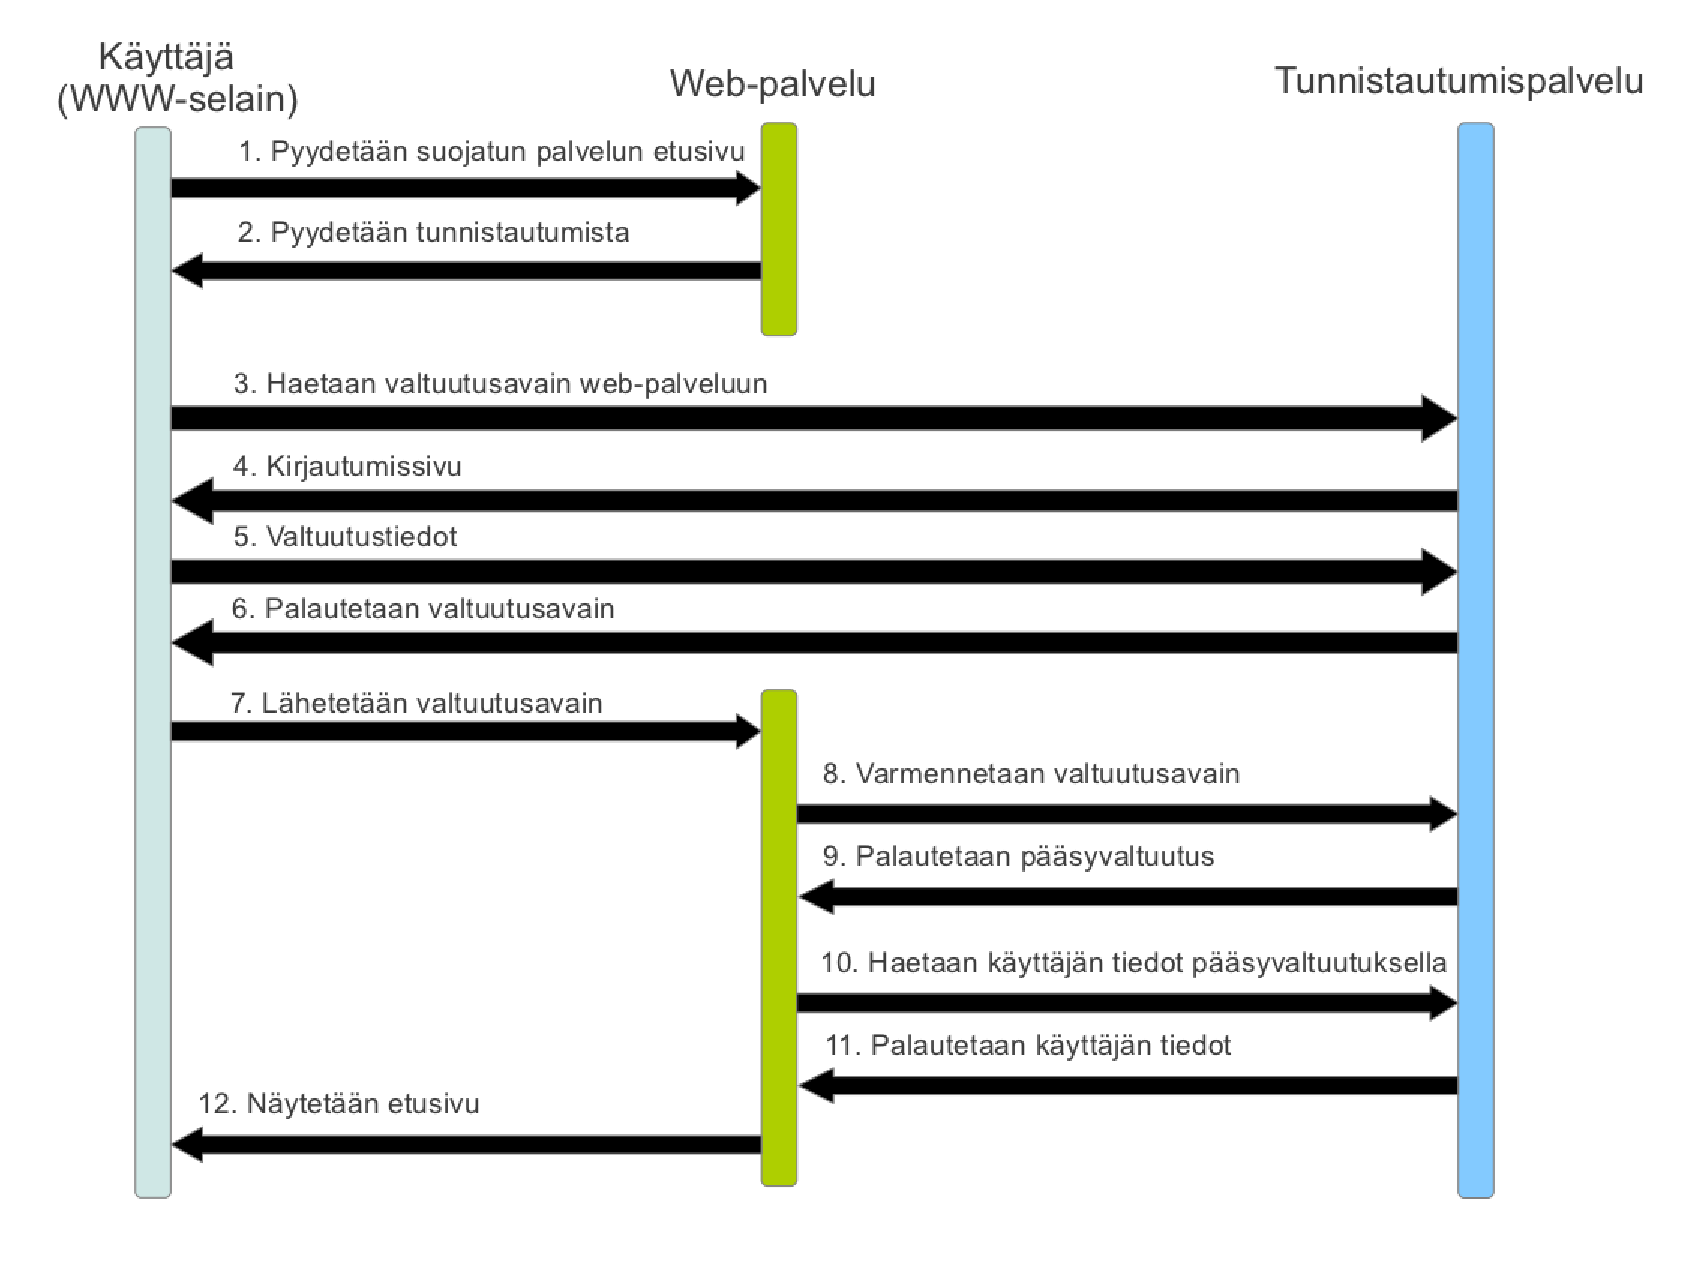
\includegraphics[width=\textwidth]{teknologiat/protokollat/oauth.eps}
\caption{OAuth sekvenssikaavio}%
\label{oauth}
\end{figure}

\subsection{Vertailu (rajapinnat ja käyttäjädata)}
Käytetään OAuthia protossa, koska OpenID:ssä kaikkea tarpeetonta mukana. SAML taas skipataan, koska...? Tätä pitäisi pohtia jossain kohtaa.